\documentclass{jlreq}
\usepackage{graphicx}
\usepackage{amsmath,amssymb,mathtools,bm}
\usepackage{siunitx}
\sisetup{per-mode=symbol}
\usepackage{physics}
\usepackage{mhchem}
\usepackage{booktabs}
\usepackage{ascmac}
\usepackage{hyperref}
\hypersetup{colorlinks=true,linkcolor=black,urlcolor=blue,citecolor=black}
\usepackage{enumitem}
\usepackage{geometry}
\usepackage{caption}
\usepackage{makecell} % ← セル内改行・回転文字用
\usepackage{multirow}
\usepackage{diagbox}

% ===== Title =====
\title{質点系の重心}
\author{学籍番号：2225091~~~~~~氏名 : 西亦 岳雄}

\begin{document}

\maketitle




% ===== 目的 =====
\section*{1.目的}
今回の実験では, 「アクリル板とおもりを用いた重心の測定」, 
「積み重ねた板材のせり出しの実験」,「やじろべえの安定性の実験」において, 
複数の質点が構成する質点系の重心を求め, 実験値と計算値を比較検討する.



% ===== 原理 =====
\section*{2.原理}
多数の質点からなる質点系全体の質量中心を重心という. 系全体の質点各々について, 
その系の全質量がその中心にあるかのように運動する. \par

$n$個の質点からなる質点系の重心は, $i$番目の質点の位置ベクトルを$\bm{r}_i$
, 質量を$m_i$とすると
\begin{align}
    \bm{r}_G = \frac{\sum m_i \bm{r}_i}{M}
\end{align}
と書ける. ($M$は質点系全体の質量で, $\sum m_i$.) 各々の質点の
$x,y,z$座標軸の成分を用いて, 重心の座標を表すと
\begin{align}
    x_G = \frac{\sum m_i x_i}{\sum m_i},　y_G = \frac{\sum m_i y_i}{\sum m_i},　z_G = \frac{\sum m_i z_i}{\sum m_i}.
\end{align}



% ===== アクリル板とおもりを用いた重心の測定 =====
\section*{3.アクリル板とおもりを用いた重心の測定}


% ===== 実験装置構成・方法 =====
\subsection*{3.1.実験装置構成・方法}

はじめに, 質量を測定した5個のおもりをアクリル板上に設置し, その重心を求めた. 
その後, 重心を求めたおもりの設置位置について, 重心の位置を計算で求めた. 
その後, 実験値と計算値を比較し検討した. 

図1のように支棒を鉛筆として, 5つのおもりを乗せたアクリル板
を支えた. アクリル板が滑り落ちるのを防ぐため, 消しゴム付き鉛筆を
用いて支えた. アクリル板には図のように格子が描かれており, この格子の
交点を重心の座標計算に用いる. 


\begin{figure}[hbtp]
  \centering
  
\includegraphics[width=0.9\linewidth]{images/number1.png} % ← 拡張子・大文字小文字に注意！
  \caption{アクリル板とおもり及び鉛筆を用いた実験装置}
\end{figure}










% ===== 結果・解析 =====
\subsection*{3.2.結果・解析}

\subsubsection*{3.2.1.　1回目の重心計測}


\begin{figure}[hbtp]
  \centering
  
\includegraphics[width=0.9\linewidth]{images/number2.png} % ← 拡張子・大文字小文字に注意！
  \caption{1回目の重心計測}
\end{figure}

1回目の重心計測では, 図2のように5つのおもりを配置した. 
5つのおもりをそれぞれA,B,C,D,Eとし, その質量は電子はかり
で測ったところ$m_\text{A} = 50.39$g, $m_\text{B} = 50.99$g,
 $m_\text{C} = 50.67$g, $m_\text{D} = 49.92$g, 
 $m_\text{E} = 43.32$gであった(2回目の重心計測も同様). 
 図2は1回目の測定を表したもので, 
 スマートフォンで撮影した写真を再現したものである.
  おもりにはそれぞれA,B,C,D,Eと
名前を振ってあり, 原点は赤点, 実験のおける重心は黒点, 
理論計算における重心は水色点で表した. \par

1回目の重心計算では図2のように$x-y$軸をおき, 
原点の座標(0,0)を手前から見てアクリル板の左端に置いた. 
これより, おもりA~Bの座標はA(1,5), B(7,9), C(5,1), D(1,1), E(9,3)
となる. \par

おもりの各質量と各座標から理論重心を求めると, おもりの合計質量は
\begin{align}
    M = 50.39+50.99+50.67+49.92+43.32 = 245.29\text{(g)}.
\end{align}
また, (2)から$x,y$座標に関して

\begin{align}
    \sum m_i x_i &= 50.39 \times 1 + 50.99 \times 7 + 50.67 \times 5 + 49.92 \times 1 + 43.32 \times 9\\
                 &= 1100.47
\end{align}

\begin{align}
    \sum m_i y_i &= 50.39 \times 5 + 50.99 \times 9 + 50.67 \times 1 + 49.92 \times 1 + 43.32 \times 3\\
                 &= 941.41
\end{align}
であるから, 

\begin{align}
    x_G = \frac{\sum m_i x_i}{M} = \frac{1100.47}{245.29} \approx 4.49
\end{align}

\begin{align}
    y_G = \frac{\sum m_i y_i}{M} = \frac{941.41}{245.29} \approx 3.84
\end{align}

で理論重心の位置は$(x_G,y_G)_{理論} \approx (4.49,3.84)$と分かった. 
また, 図2から実験重心はおよそ$(x_G,y_G)_{実験} \approx (5.00,4.30)$
とわかった. 
これをまとめたものが以下の表1である. 


\begin{table}[htbp]
  \centering
  \caption{アクリル板と錘の重心}
  \begin{tabular}{|c|c|c|}
    \hline
    おもり & 質量 (g) & 位置座標 \\
    \hline
    $m_{\mathrm{A}}$ & 50.39 & $(x,y) = (1,5)$ \\
    \hline
    $m_{\mathrm{B}}$ & 50.99 & $(x,y) = (7,9)$ \\
    \hline
    $m_{\mathrm{C}}$ & 50.67 & $(x,y) = (5,1)$ \\
    \hline
    $m_{\mathrm{D}}$ & 49.92 & $(x,y) = (1,1)$ \\
    \hline
    $m_{\mathrm{E}}$ & 43.32 & $(x,y) = (9,3)$ \\
    \hline
    アクリル板 & 139.84 &  \\
    \hline
    \multicolumn{2}{|c|}{実験で得た重心位置} &
      $(x_G,y_G) = (5.00,\,4.30)$ \\
    \hline
    \multicolumn{2}{|c|}{計算で得た重心位置} &
      $(x_G,y_G) = (4.49,\,3.84)$ \\
    \hline
  \end{tabular}
  \label{tab:cg_acrylic}
\end{table}



\subsubsection*{3.2.2.　2回目の重心計測}

2回目の重心計測では, 図3のように5つのおもりを設置した. 
おもりの名前と質量は1回目の重心計測のときと同じで, 2回目もスマートフォンで
撮影した写真を図として再現した. \par

2回目の重心計測では, $x-y$軸及び原点(0,0)は図3のように設定した.
これより, 各おもりの座標はA(7,9), B(7.3), C(9,1), D(3,1), E(3,5)
となる. \par



\begin{figure}[hbtp]
  \centering
  
\includegraphics[width=0.9\linewidth]{images/number3.png} % ← 拡張子・大文字小文字に注意！
  \caption{2回目の重心計測}
\end{figure}


おもりの各質量と各座標から理論重心を求める. おもりの合計質量は(3)式
より$M = 245.29$(g).
また, (2)から$x,y$座標に関して

\begin{align}
    \sum m_i x_i &= 50.39 \times 2 + 50.99 \times 2 + 50.67 \times 4 + 49.92 \times (-2) + 43.32 \times (-2)\\
                 &= 218.96
\end{align}

\begin{align}
    \sum m_i y_i &= 50.39 \times 4 + 50.99 \times (-2) + 50.67 \times (-4) + 49.92 \times (-4) + 43.32 \times 0\\
                 &= -302.78
\end{align}
であるから, 
\begin{align}
    x_G = \frac{\sum m_i x_i}{M} = \frac{218.96}{245.29} \approx 0.893
\end{align}

\begin{align}
    y_G = \frac{\sum m_i y_i}{M} = \frac{-302.78}{245.29} \approx -1.23
\end{align}


で理論重心の位置は$(x_G,y_G)_{理論} \approx (0.89,-1.23)$と分かった. 
また, 図3から実験重心はおよそ$(x_G,y_G)_{実験} \approx (0.75,-0.90)$
とわかった. 
これをまとめたものが以下の表2である. 




\begin{table}[htbp]
  \centering
  \caption{アクリル板上の質点と重心}
  \begin{tabular}{|c|c|c|}
    \hline
    おもり & 質量 (g) & 位置座標 \\
    \hline
    $m_1$ & 50.39 & $(x,y) = (2,4)$ \\
    \hline
    $m_2$ & 50.99 & $(x,y) = (2,-2)$ \\
    \hline
    $m_3$ & 50.67 & $(x,y) = (4,-4)$ \\
    \hline
    $m_4$ & 49.92 & $(x,y) = (-2,-4)$ \\
    \hline
    $m_5$ & 43.32 & $(x,y) = (-2,0)$ \\
    \hline
    アクリル板 & 139.84 &  \\ % 空欄のまま
    \hline
    \multicolumn{2}{|c|}{実験で得た重心位置} &
      $(x_G,y_G) = (0.75,\,-0.90)$ \\
    \hline
    \multicolumn{2}{|c|}{計算で得た重心位置} &
      $(x_G,y_G) = (0.89,\,-1.23)$ \\
    \hline
  \end{tabular}
  \label{tab:acrylic_cg}
\end{table}




% ===== 考察 =====
\subsection*{3.3.考察}

1回目のおもりの配置では, 理論重心と実験重心の差は$x \approx 0.5$,
$y \approx 0.5$程度で小さいズレとなり, 2回目のおもりの配置においても
$x,y$それぞれ0.1~0.3程度の差となり理論値と実験値は概ね一致したと言える.\par

完全な一致とならなかったのは, アクリル板の質量を考慮していないこと, 
鉛筆に取り付けてある消しゴムはアクリル板との間に摩擦を生みやすく
本来であれば支えきれないものを支えることができたことが考えられる. 







% ===== 積み重ねた板材のせり出しの実験 =====
\section*{4.積み重ねた板材のせり出しの実験}

% ===== 実験装置構成・方法 =====
\subsection*{4.1.実験装置構成・方法}



はじめに, 形状と質量が近しい板材を6枚選び, 1番上の板が支えている端から
板1枚分以上せり出すように板を重ねた. その後, 各板のせり出した距離を
求め, 併せてせり出しの理論最大値を求めた. \par

図4が実験装置で, 板材は上から順にA,B,C,D,E,Fとし, 各質量は順に
A:129.10g, B:124.69g, C:130.96g, D:128.26g, E:131.07g
で, 板材の長さはおよそ36cmであった. 



\begin{figure}[hbtp]
  \centering
  
\includegraphics[width=1.0\linewidth]{images/number4.png} % ← 拡張子・大文字小文字に注意！
  \caption{積み重ねた板材}
\end{figure}


\begin{figure}[hbtp]
  \centering
  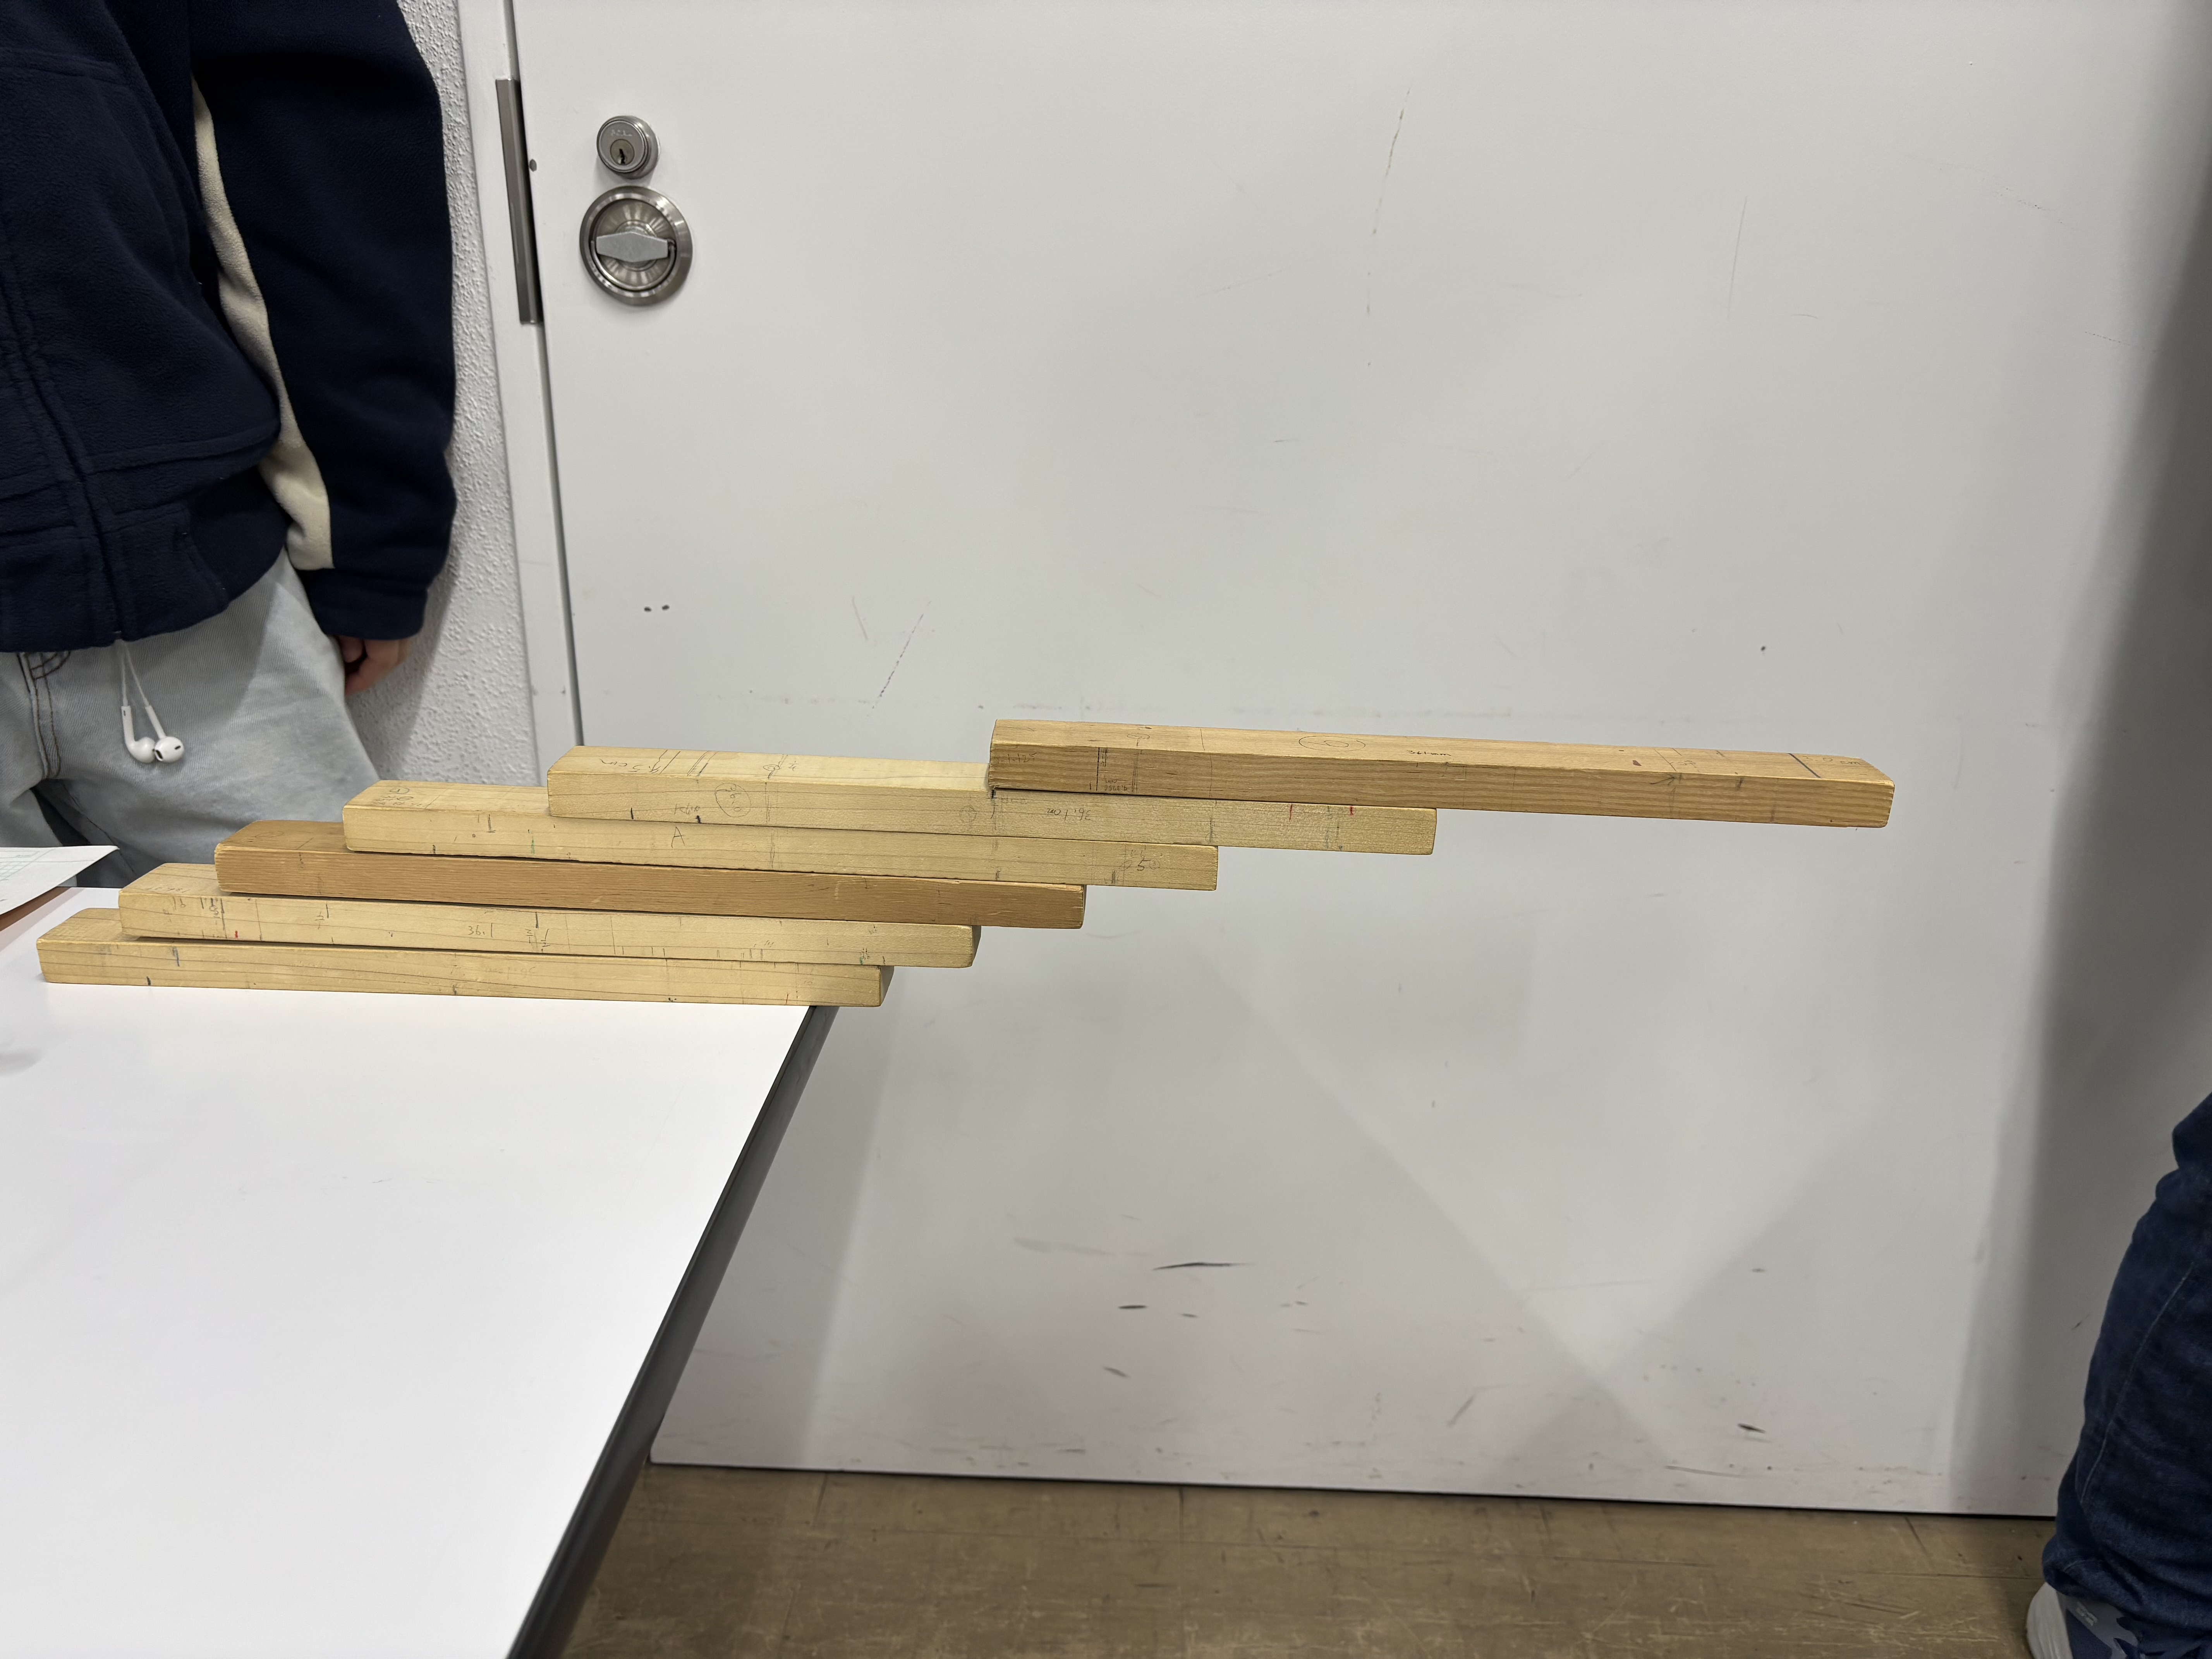
\includegraphics[width=0.5\linewidth]{images/number5.jpg} % ← 拡張子・大文字小文字に注意！
  \caption{積み重ねた板材(実際の写真)}
\end{figure}

\vspace{20mm}
% ===== 結果・解析 =====
\subsection*{4.2.結果・解析}

各板はすぐ下の板より右側へ距離$d_\text{A}, d_\text{B}, \dots , d_\text{F}$
だけせり出している. 一般に, 上から$n$番目の板がすぐ下の$n+1$番目の板より
距離$d_n$だけ前にせり出して静止しているとする. 
このとき, $n$番目の板の上には$n-1$枚の板が乗っているので, 
$n-1$枚の板全体の重心が$n$番目の板の左端の真上にくるとき, 
板が崩れる限界となる. \par

$n+1$番目の板の左端の周りの力のモーメントのつり合いを考えると
\begin{align}
    (n-1)mg\,d_n \leq mg\!\left(\frac{a}{2}-d_n\right)
\end{align}
が成り立つ. 両辺を$mg$で割って, $d_n$について整理して
\begin{align}
    (n-1)d_n \leq \frac{a}{2}-d_n
 \quad\Rightarrow\quad
 nd_n \leq \frac{a}{2}
 \quad\Rightarrow\quad
 d_n \leq \frac{a}{2n}
\end{align}
を得る. \par

今回の実験で用いた6枚の板に関して, 上から順に
\begin{align}
    \text{板 A（$n=1$）}:&\quad d_{\mathrm{A}} \leq \frac{a}{2}
   = \frac{36}{2} = 180\ \mathrm{mm},\\
\text{板 B（$n=2$）}:&\quad d_{\mathrm{B}} \leq \frac{a}{4}
   = 90\ \mathrm{mm},\\
\text{板 C（$n=3$）}:&\quad d_{\mathrm{C}} \leq \frac{a}{6}
   = 60\ \mathrm{mm},\\
\text{板 D（$n=4$）}:&\quad d_{\mathrm{D}} \leq \frac{a}{8}
   = 45\ \mathrm{mm},\\
\text{板 E（$n=5$）}:&\quad d_{\mathrm{E}} \leq \frac{a}{10}
   = 36\ \mathrm{mm},\\
\text{板 F（$n=6$）}:&\quad d_{\mathrm{F}} \leq \frac{a}{12}
   = 30\ \mathrm{mm}
\end{align}
となる. したがって, テーブルの縁から一番上の板Aの右端までの
理論最大せり出し距離$D_{\max}$は

\begin{align}
    D_{\max} = d_{\mathrm{A}}+d_{\mathrm{B}}+d_{\mathrm{C}}
          +d_{\mathrm{D}}+d_{\mathrm{E}}+d_{\mathrm{F}}
          = 441\ \mathrm{mm}
\end{align}
と推測できる. \par

以下の表3は板A~Fまでのせり出し距離を実測値と理論値でまとめたものである.
実験値でのせり出し距離合計は440mmであったが, 理論値のそれは
441mmとなった. 


\begin{table}[htbp]
  \centering
  \caption{板のせり出し距離の実験値と計算値}
  \begin{tabular}{|c|c|c|c|c|}
    \hline
    \multirow{2}{*}{$n$ 番目の板} &
      \multicolumn{2}{c|}{実験 (mm)} &
      \multicolumn{2}{c|}{計算 (mm)} \\ \cline{2-5}
    & せり出した距離 & せり出し距離合計 &
      せり出した距離 & せり出し距離合計 \\
    \hline
    1 (A) & 178 & 440 & 180 & 441 \\
    \hline
    2 (B) &  87 & 262 &  90 & 261 \\
    \hline
    3 (C) &  62 & 175 &  60 & 171 \\
    \hline
    4 (E) &  45 & 113 &  45 & 111 \\
    \hline
    5 (D) &  37 &  68 &  36 &  66 \\
    \hline
    6 (F) &  31 &  31 &  30 &  30 \\
    \hline
  \end{tabular}
  \label{tab:overhang_result}
\end{table}
   




% ===== 考察 =====
\subsection*{4.3.考察}

実験値は理論式より少し小さく出ている. これは, 板の長さを全て36cm
と理想的な状態にしたこと, 板の質量を全て等しいとしたこと, 
また板とテーブルとの摩擦, 板同士の摩擦による理論値で考慮していない
力が加わっていること, 板が僅かに反っていること, 厚みや密度が一様でないこと
に起因するものと考えられる. \par

しかし, 理論値とは1mm程度しか差異がなく, 各板のせり出し距離も理論値に
非常に近くなった. これは, 上から$n$番目の板の重心が下の板の左端を
超えないという条件においては, (17)式が近似式として有意であることを示している.






% ===== やじろべえの安定性の実験 =====
\section*{5.やじろべえの安定性の実験}


% ===== 実験装置構成・方法 =====
\subsection*{5.1.実験装置構成・方法}

はじめに, 大きさの異なる2種類の木球, 細い木の棒, 木球固定用の
ゴムリングを用いて重心を高くしたときでもなるべく安定するような
やじろべえを作成した. その際に, 各パーツの重量も電子はかりで計測した.
「アクリル板とおもりを用いた重心の測定」で用いたアクリル版を使い, 
各パーツの質量と位置関係から重心の位置を推測した. このとき, ゴムリング
の質量は非常に僅かであるため考慮しなかった. 次に, 中心の木球の支点からの
位置$x$を少しずつ大きくしていき, 支点と中心の木球の位置に対する
やじろべえの軸の傾きとの関係を測定し, 推測した重心の位置と比較をした.
軸の傾きはスマートフォンでやじろべえを撮影し, 
写真から分度器を用いて計測した. \par

以下の図6はやじろべえの実験装置構成で, 
やじろべえは木台の上に安定させて設置し, 木球の中心と支点との距離は
$x = 2.7$cmであった. また, 各パーツの質量は, 左右の木球はそれぞれ
16.00g, 16.07g, 小さな木球は5.32g, 左右の木棒はそれぞれ
1.55g, 1.52g, 真ん中の長い木棒は1.83gで, やじろべえの合計質量は
42.29g.



\begin{figure}[hbtp]
  \centering
  
\includegraphics[width=0.6\linewidth]{images/number6.png} % ← 拡張子・大文字小文字に注意！
  \caption{やじろべえの概観}
\end{figure}



% ===== 結果・解析 =====
\subsection*{5.2.結果・解析}
図7にあるように, アクリル板を用いて計測したやじろべえの重心(理論重心)は\par
合計質量
\begin{align}
    M = 16.00 + 16.07 + 5.32 + 1.55 + 1.52 + 1.83 = 42.29\text{g}
\end{align}
と
\begin{align}
    \sum m_i x_i &= 16.00 \times 0 + 16.07 \times 10 + 5.32 \times 5 + 1.55 \times 2.5 + 1.52 \times 7.5 + 1.83 \times 5 \\
    &= 211.73
\end{align}
\begin{align}
    x_G = \frac{\sum m_i x_i}{M} \approx \frac{211.73}{42.29} \approx 5.01
\end{align}
及び
\begin{align}
    \sum m_i y_i &= 16.00 \times 6 + 16.07 \times 6 + 5.32 \times 3 + 1.55 \times 4.5 + 1.52 \times 4.5 + 1.83 \times 3 \\
    &= 227.69\text{g}
\end{align}
\begin{align}
    y_G = \frac{\sum m_i y_i }{M} \approx \frac{227.69}{42.29} \approx 5.38
\end{align}
で, 棒の質量を無視する近似のもとでのやじろべえの重心は
\begin{align}
    (x_G,y_G) \approx (5.0,5.4)
\end{align}
となった.



ここからは, 支点と木球の中心の位置に対するやじろべえの軸の傾き角度との
関係から重心の位置を推測する. 以下の図7は, やじろべえが傾いたときの
概観である. 


\begin{figure}[hbtp]
  \centering
  
\includegraphics[width=0.4\linewidth]{images/number7.png} % ← 拡張子・大文字小文字に注意！
  \caption{傾いたときのやじろべえ}
\end{figure}


以下の表4が実際の軸の傾きと支点と木球の中心距離の数値である.


\begin{table}[htbp]
  \centering
  \caption{支点位置とやじろべえ軸の傾きの測定結果}
  \begin{tabular}{|c|c|}
    \hline
    支点と木球中心との距離 (m) & 軸の傾き $\theta$ (°) \\
    \hline
    0.000 & 0  \\
    \hline
    0.027 & 0  \\
    \hline
    0.037 & 10 \\
    \hline
    0.042 & 20 \\
    \hline
    0.043 & 60 \\
    \hline
    0.044 & 67 \\
    \hline
    0.045 & 82 \\
    \hline
    0.046 & 85 \\
    \hline
    0.047 & 92 \\
    \hline
  \end{tabular}
  \label{tab:yajirobe_pivot_angle}
\end{table}

また, 表4の数値をプロットしたものが図8で, 支点と木球の中心との距離$x$が
$x$ = 0.043mのとき急激にやじろべえが傾くことがわかる. 
これは, 支点が重心を超えることでやじろべえが不安定になったことを示し,
よってやじろべえの重心は$x_G \approx 0.043$mの近くにあるとわかる.



\begin{figure}[hbtp]
  \centering
  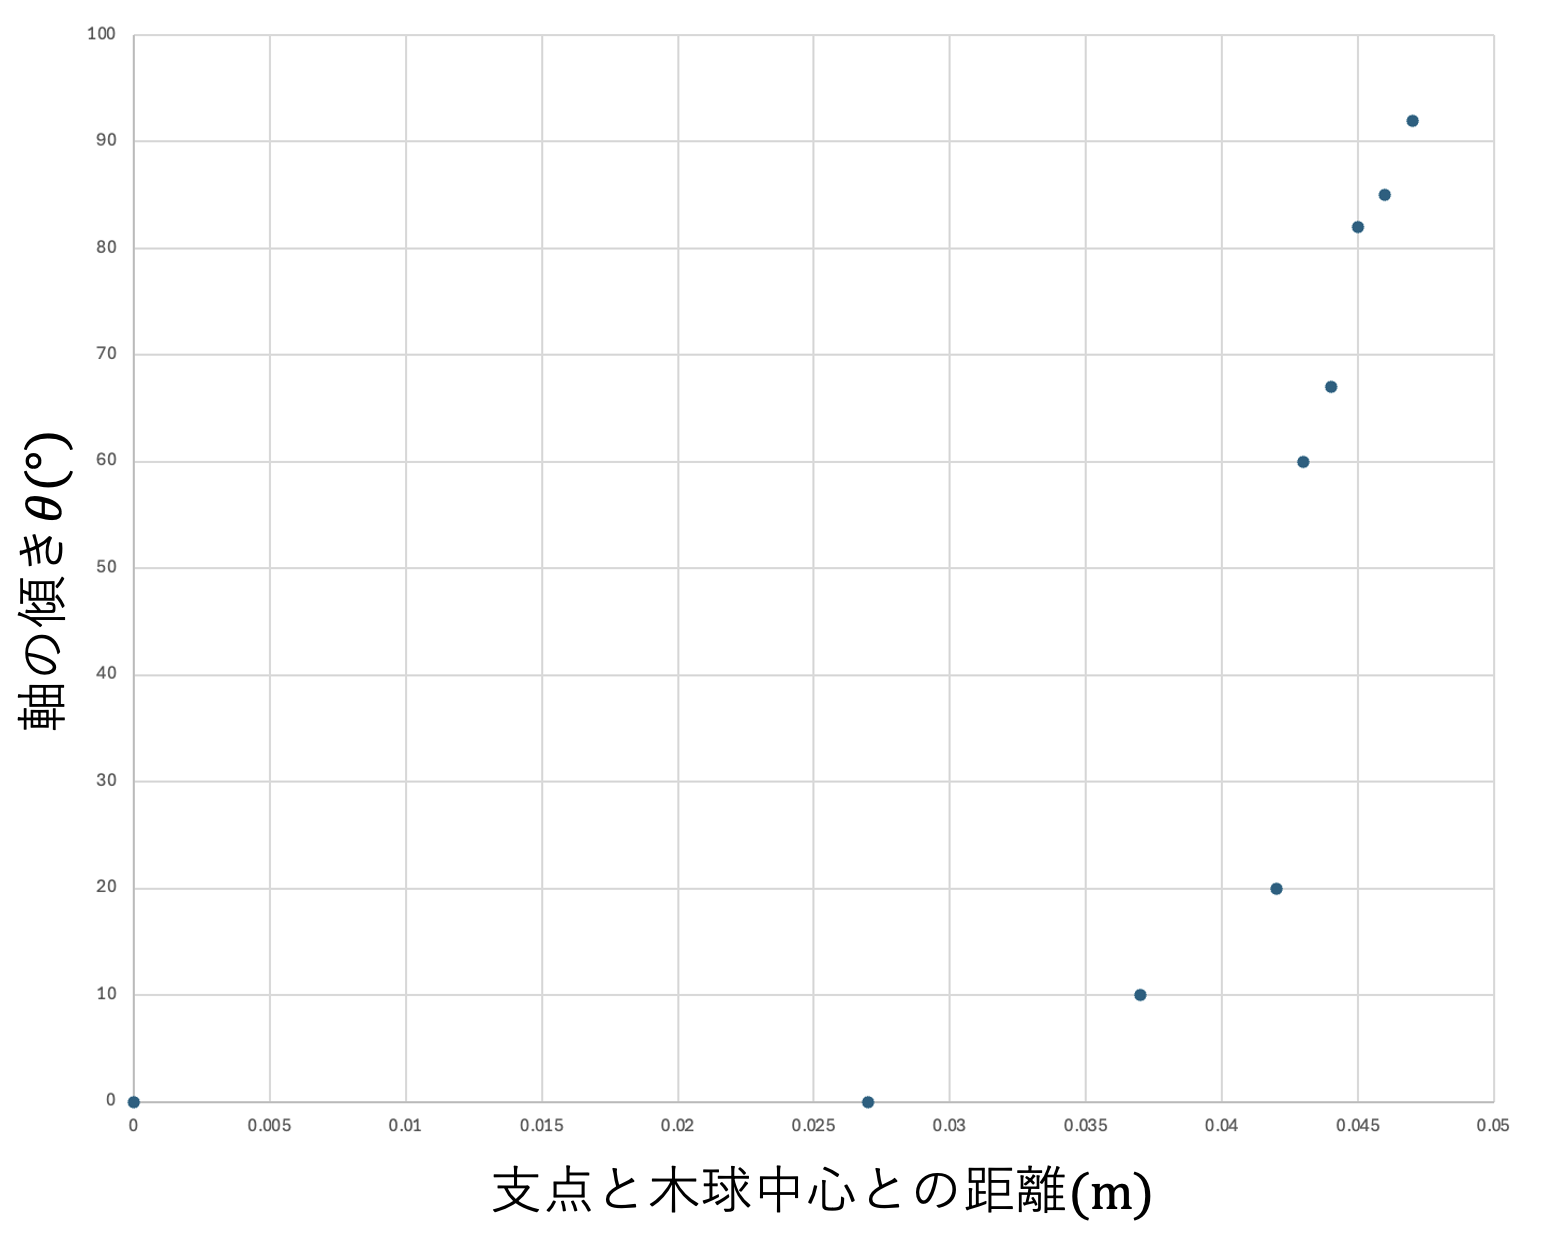
\includegraphics[width=1.0\linewidth]{images/number8.png} % ← 拡張子・大文字小文字に注意！
  \caption{支点位置とやじろべえ軸の傾きの関係}
\end{figure}





% ===== 考察 =====
\subsection*{5.3.考察}
今回の実験では, 左右の木球と木棒で構成されたやじろべえを用いて,
支点と小さい木球の中心の距離$x$を変化させ軸の傾き$\theta$を計測した.
その結果, 図8からわかるように, $x$が0.003mに満たないときは
$\theta \approx 0$とおおかた鉛直に保たれていたが, $x \approx 0.043$m
あたりから急激に$\theta = 60$以上に増加することがわかった. 
これは, 支点の位置がやじろべえの重心の鉛直下からずれ込むと, 微細な
変位でもやじろべえにかかる重力モーメントが大きくなり, 
傾きが大きくなることを示す. プロットからは, $x = 0.042$と$x = 0.044$
の間に安定が崩れる境界があり, 図9を見ても理論重心との差はわずかとわかる.

この差は, ゴムリングの質量を無視したこと, 支点と木球中心との距離
の読み取りに数mmの差異があること, 支点と木台の摩擦でやじろべえにかかる
トルクに影響して安定する状態に変化を与えていることが考えられる. 



\begin{figure}[hbtp]
  \centering
  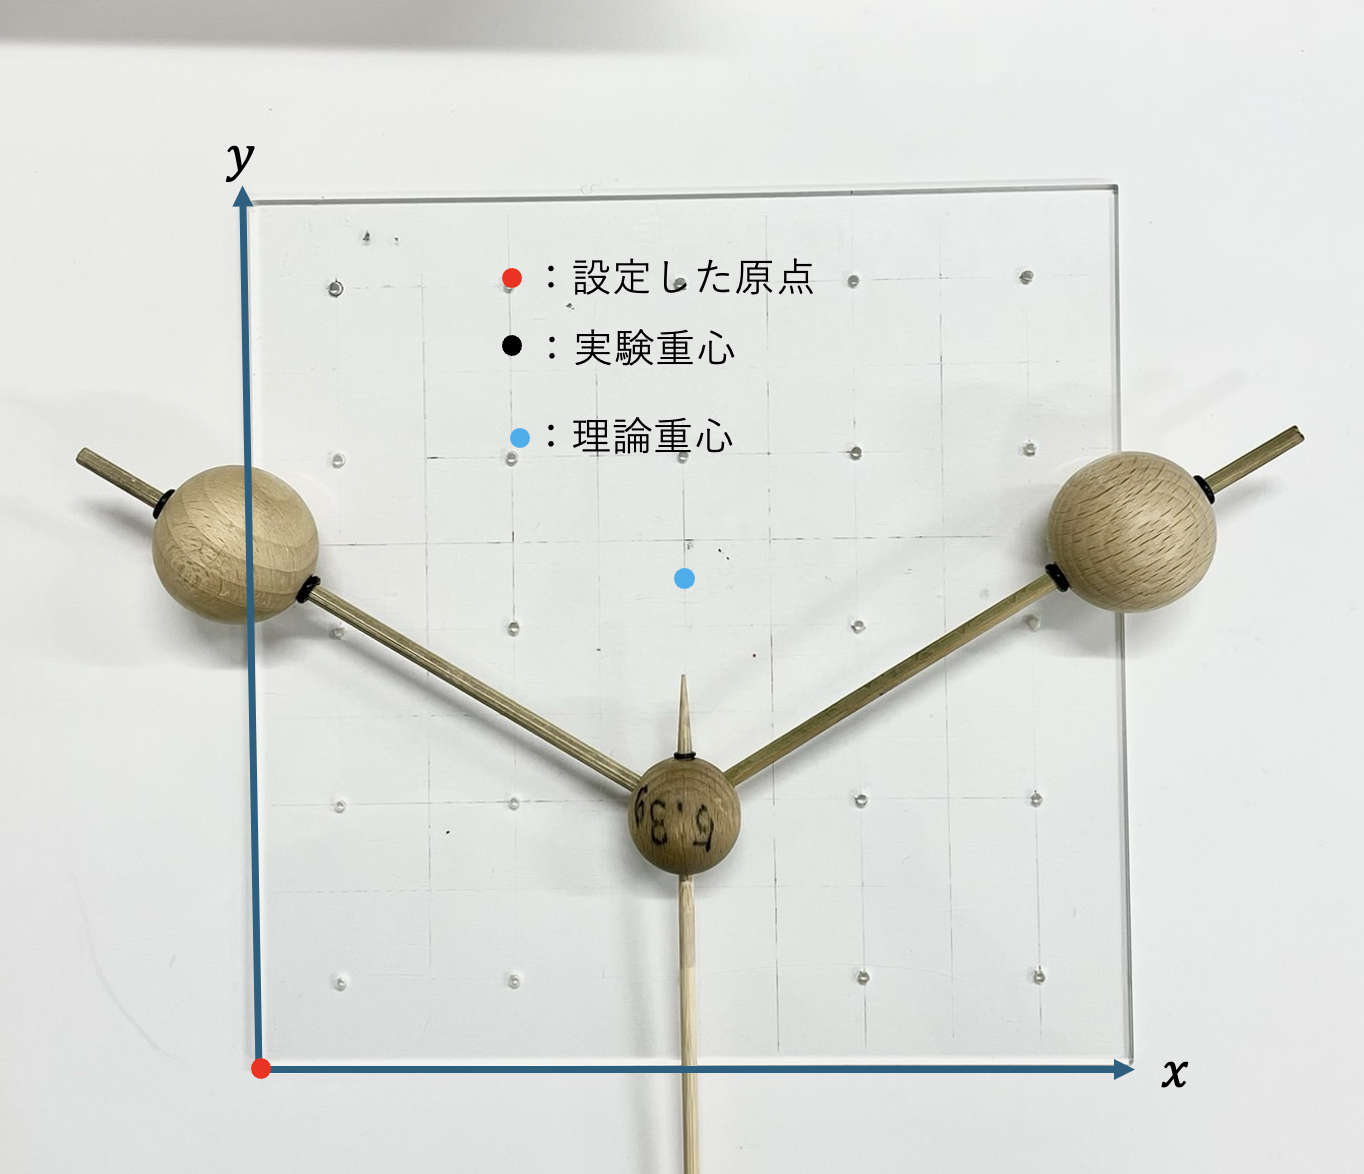
\includegraphics[width=0.8\linewidth]{images/number9.png} % ← 拡張子・大文字小文字に注意！
  \caption{重心の位置}
\end{figure}




\section*{6.まとめ}
3つの実験において, 質点系と剛体, またその複合的な状況に対して
重心が安定する条件の大きな要素であることがわかった. また, アクリル板や木棒の質量を
どう扱って支点や目盛りの差異をどれくらい見積もるのかという近似の仕方
が理論と実験の差異として現れることを理解できた.






\begin{thebibliography}{9}

\bibitem{gyro-text}
東京理科大学基礎物理学実験テキスト編集委員会：
『基礎物理学実験　入門編』，内田老鶴囲，2016．



\end{thebibliography}


\end{document}